
% CHAPTER 2

\chapter{LITERATURE SURVEY}
\label{chp:Literature Survey}

\externaldocument{chapter1}
\externaldocument{chapter6}
\externaldocument{chapter3}
\externaldocument{chapter4}
\externaldocument{chapter5}

Formation control requires local positioning, detection of the general shape, task allocation to individual agents and task dispatching. The literature has related works in these different fields but lacks the adaptation to dynamically changing shapes. This chapter is intended to motivate the need for the topic of this thesis by underlying the gap, it has filled by reviewing existing works in related fields. 

\section{Formation Control Systems}
Formation control problem have different subproblems like formation shape generation, formation reconfiguration$\&$selection and formation tracking \cite{12}.  
In formation shape generation, agents are expected to get a formation shape which can be defined by external commands or with some mathematical constraint functions \cite{16}.  One general approach is to consider artificial potential functions. Samitha and Pubudu \cite{17} have presented an artificial potential function method  based on the consideration of the problem as controlling the position of a swarm into a shape, bounded by a simple closed contour. This approach results in deploying uniformly of swarm agents within the contour.  Their work provides analysis about the stability and robustness of the proposed system based on Lyapunov like functions. Figure \ref{samitha_obstacle} illustrates a simulation environment of a swarm getting the desired pentagonal like formation shape in presence of obstacles. Here the desired formation shapes is defined with an analytical expression and individual control laws for agents are composed with artificial potential functions using these analytical expressions. In real world applications, it may not be possible to have the analytical expressions of the desired formation shape. In our thesis work, we have focused on designing control laws which do not depend on the analytical expressions of the formation shapes.

\begin{figure}[H]
	\caption{Motions and Formation of the Agents in Presence of Obstacles \cite{17}} \label{samitha_obstacle}
	\centering
	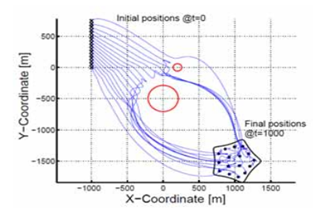
\includegraphics[scale = 0.7]{samitha}
\end{figure} 

In some applications, it may be needed to change the formation shape or splitting and joining of the agents together due to either a change in coordinated task requirements or change in environmental conditions such as narrow corridors. In such a scenario, the swarm has to propagate in a narrow corridor before reaching the desired goal state and it is not possible to follow this path by keeping the final desired formation shape. Hence, swarm has to adapt itself to environmental conditions while following a predetermined trajectory. This task requires formation reconfiguration and dynamic task assignment of swarm agents to be dispatched. Hou et al. \cite{8} have defined a method based on global objective functions to provide formation control of a swarm. In their approach it is possible to implement scaling and rotating functions into control laws to adapt the swarm to environmental conditions while achieving a specific task. 

\begin{figure}[H]
	\caption{A Swarm in Rotating and Scaling Ellipse Formation \cite{8}} \label{slotine_fig_ref}
	\centering
	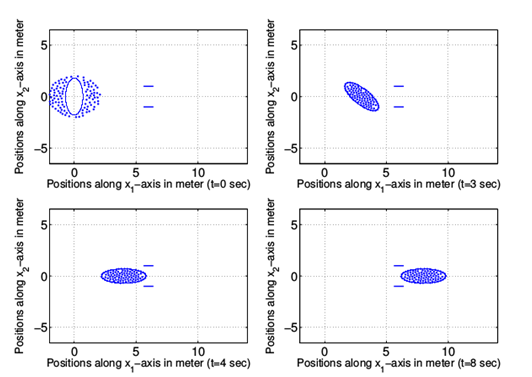
\includegraphics[scale = 1]{slotine}
\end{figure} 

Figure \ref{slotine_fig_ref} illustrates a simulation environment with a swarm of 100 mobile agents with an ellipsoidal formation shape. The formation shape is rotated dynamically to follow a path through a narrow corridor. Swarm has to adapt this  rotation maneuver to follow the desired trajectory. This kind of dynamical adaptations are always required in complex tasks in real time applications with complicated workspaces. Their approach also requires the analytical expressions for the desired formation shapes.

One of the subproblems studied in formation control is formation tracking. The main objective of this problem is to maintain a desired formation with a group of robots, while tracking or following a reference trajectory. The solutions for the formation tracking approaches can be classified into three basic strategies as leader-following, virtual structure and behaviour based approaches \cite{12}. The most general strategy to provide a solution for this problem is leader-following swarm structures \cite{18}. Other strategies have a basis on optimization and graph theory approaches \cite{12}. Kumar et al. proposed a vision based formation control framework  for this problem. This framework has a leader following infrastructure \cite{18}. Figure \ref{Kumar_Ferrro} illustrates a simulation environment of this leader follower approach on formation tracking problem. The individual agents achieve a coordinated turn by keeping their relative positions to their local neighbors. 

\begin{figure}[H]
	\caption{Five Robot Formation With Trajectory Tracking \cite{18}} \label{Kumar_Ferrro}
	\centering
	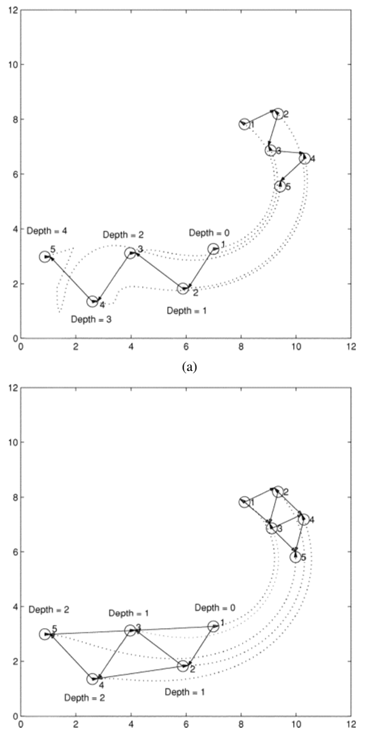
\includegraphics[scale = 0.65]{kumar}
\end{figure} 


In leader following strategy, some of the agents in the swarm are the leaders to manage the rest of the swarm to achieve a desired specific task and the rest of the agents act as followers. This approach reduces the formation control problem into tracking control problem of individuals to follow the leader from a desired distance and bearing angle, thus the stability and convergence analysis of the formation can be done with the usage of single tracking controllers of members. This approach simplifies the tracking problem of a network of agents to a single agent. Kumar et al. at \cite{18} proposed a control framework in which follower agents move along a trajectory afterwords the leader agent with a desired separation distance $l_{ij}$ and desired relative bearing angle $\psi_{ij}$.  Figure \ref{leader_follower_ref} represents a formation control with three agents where R3 is the leader and R1,R2 are the follower agents. 

\begin{figure}[H]
	\caption{Leader-Follower Systems \cite{18}} \label{leader_follower_ref}
	\centering
	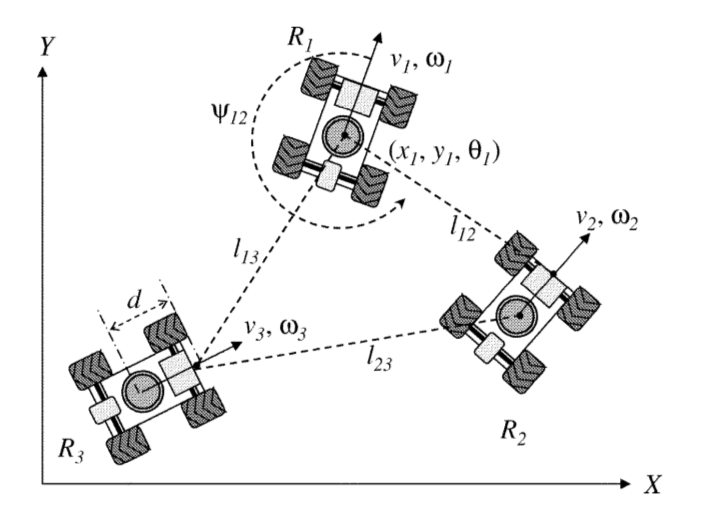
\includegraphics[scale = 0.5]{leader}
\end{figure}


In this approach it is hard to gather the agents in a certain shape. Another drawback is that, determining the separation and bearing angles for individual agents is getting harder as the number of agents in the swarm increases and this strategy is not fault tolerant to the absence of communication between agents.


In virtual structure approach, the formation is composed with a virtual rigid body. Formation control is applied to the whole virtual structure and then the individual agent control laws are determined with inverse dynamic solutions \cite{12}.  Lewis and Tan \cite{23} proposed a virtual structure based method for formation control  with a bidirectional flow control where robots move to keep the virtual structure when the swarm is following a trajectory and virtual structure adapt itself to the robots' current positions to compensate the relative errors at the end of a maneuver. Figure \ref{virtual_structir} illustrates such a maneuver implemented with their approach.

\begin{figure}[H]
	\caption{Maneuver of a Formation and Compensation of Virtual Structure} \label{virtual_structir}
	\centering
	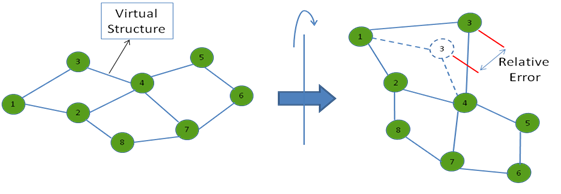
\includegraphics[scale = 0.95]{virtual_structure}
\end{figure}

In virtual structure strategy it is easy to achieve a coordinated behaviour for the group to maintain the formation during a trajectory tracking or a maneuvering, but it is not a suitable strategy to apply a formation control to achieve certain geometrical shape with the swarm agents. 


Behaviour based strategies model every agents' behaviours to achieve specific tasks with swarm. These behaviours may be very simple like randomly walk and avoidance of  obstacles in the environment or they may be defined in a very complicated manner in order to achieve complex formation shapes with the entire swarm while for example optimizing the overall energy consumption depending  upon the implementation of the controller structures.  One of the main usage of this strategy is artificial potential field based implementations . Cheng and Nagpal have introduced a robust and self repairing formation control method for swarms \cite{24}. In this approach, individual control laws for the agents are defined with the artificial forces between agents themselves (to avoid collisions) and between the desired formation shape and agents. This solution provides robustness to the agent losses in the swarm during formation control and the rest of the swarm has the ability to refiil their absence in real time without changing the dynamics and the parameters of the formation controller. Because individual control laws are not dependent on the other member of the swarm. Each agent can calculate its own control input at an instant time with current formation shape and current members of the swarm and the whole swarm converge another equilibrium with current members \cite{24}. Figure \ref{izgara_ref} shows a simulation output of their work. Some of the agents from the right bottom corner of the desired formation shape are removed away from the swarm and the rest of the agents refill their absence during runtime. One of the main disadvantage of the artificial potential based approaches is that , the control forces applied to individual agents are determined instantaneously in accordance with that agent's and the other agents' positions and they cannot guarantee the optimization of the total distance travelled by the agents. Another drawback related with this type of solution is that, there is a possibility to have local minimas in the solution where an agent reaches an undesired point in configuration space under the equilibrium of different types of artificial force components. In that case the total control input acting on the agent will be zero because of cancelling force vectors which has opposite directions to each other generated by formation shape and obstacles etc. In this strategy, the solution may converge slowly to the steady state due to absence of generalized goal states for individual agents in the final formation shape. Because, there are no specific goal states for the individual agents to reach at the final configuration and they are expected to get a global equilibrium with the help of different artificial force components. 

\begin{figure}[H]
	\caption{Formation Control with Artificial Forces \cite{24}} \label{izgara_ref}
	\centering
	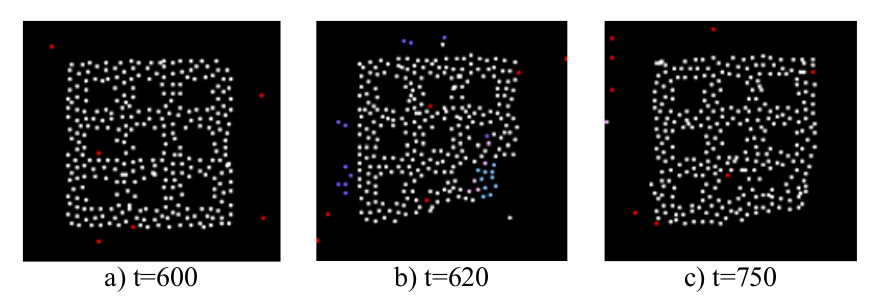
\includegraphics[scale = 0.4]{potential}
\end{figure}


Another approach is to define mathematical constraints and objective functions to achieve a specific formation shape by controlling the shape of the swarm colony while following a trajectory.  Kumar and Belta \cite{25} presented an abstraction method of configuration space to a manifold defined as $A  = G x S$ where $G$ is a lie group representing the position and the orientation of the swarm  and S represents the shape of the manifold.  They provide individual control laws which can be separately handled to manipulate the lie group $G$ to achieve formation tracking and orientation control and to manipulate the shape $S$ to achieve different geometrical shapes.Their method define the desired formation shape with shape manifold equations and control the orientation and the scale of this shape with lie group. Figure \ref{kumar_belta}
shows a simulation output in which the shape is defined as a rectangular area. The orientation and the scaling of the formation shape is dynamically changed to adapt the swarm different environmental conditions. Similarly Cheah and Slotine \cite{8} proposed a method based on objective functions . Common drawback for these researches, they can only implement a limited number of simple geometrical shapes because the desired formation shapes must be analytically identified in order to compose the related objective functions or shape manifolds. Even if it is possible to define a simple geometrical shape and to control the rotation and the scaling of this shape dynamically, there may be need for more complex and dynamically changing formation shapes rather than scaling and rotation maneuvers in real time applications. 



\begin{figure}[H]
	\caption{Formation Control with Objective Functions \cite{25}} \label{kumar_belta}
	\centering
	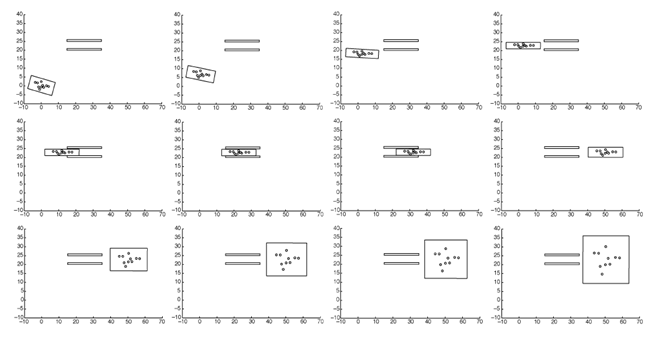
\includegraphics[scale = 0.8]{manifold}
\end{figure}



\section{Partitioning Complex Geometrical Shapes}

In this thesis work, one of the proposed solutions for the formation control problem is to partition the desired complex shapes into subsets of goal states for each type of agent in the swarm. Main idea is to dynamically assign the agents to these goal states on runtime to minimize the overall displacement of the agents. Shape partitioning process is used to determine the goal states of the agents within the formation to cover the desired complex geometrical shape. There are some different solutions in the literature including fractal filling of space algorithms and bubble$\&$circle packing algorithms. 

Fractals are self similar  patterns in all scales of themselves. They are defined with simple rules and they can cover any complex shape in the nature by progressing this simple rules iteratively. This approach is widely used in mesh generating algorithms and space filling problems.  Shier and Bourke \cite{26} have introduced a randomized fractal filling of space algorithm. They proposed a fractal based method to cover a given geometrical shape with the desired shapes and they provide the proof of their algorithm is space-filling with the following equations. Let $A$ be the total area to be filled. In our case, $A$ will be the area of the desired formation shape. If we choose the area of the fractals sequentially (i.e. bubbles which are representing the coverage area of the agents)  while filling the desired formation shape as $A_i$ with the following equation

	\begin{equation} \label{A_i_func}
	A_i = {\frac{A}{{\zeta(c,N)(i+N)^c}}}
	\end{equation}	
	
	where ${\zeta(c,N)}$ is the Hurwitz zeta function defined by 
	\begin{equation} \label{hurwitz}
	\zeta(c,N) = \sum_{i=0}^{\infty}\left(\frac{1}{(i+N)^c}\right)
	\end{equation}
	This Hurwitz zeta function will converge to zero while $i\to\infty$  with selection of $c>1$ and $N>0$. In view of Equation \ref{A_i_func} one can write by replacing the Hurwitz zeta function with the definition given in Equation \ref{hurwitz}
	\begin{equation} \label{A_i_equation}
	\sum_{i=0}^{\infty}A_i = \sum_{i = 0}^{\infty}\left(\frac{A}{\zeta(c,N)(i+N)^c}\right) = A
	\end{equation}


such that the sum of all areas $A_i$ is the total area $A$ to be filled, that is, if the algorithm does not halt then it is space-filling. Thus, it is possible to fill the desired shape with fractals chosen with areas defined in Equation \ref{A_i_equation}. Some of the outputs of their algorithm is given at Figure \ref{space_filling}. The desired shapes are filled with rectangular and star shaped fractals by selecting the areas as described in Equation \ref{A_i_equation}.



\begin{figure}[H]
	\caption{Space Filling Examples with Randomized Fractals \cite{26}} \label{space_filling}
	\centering
	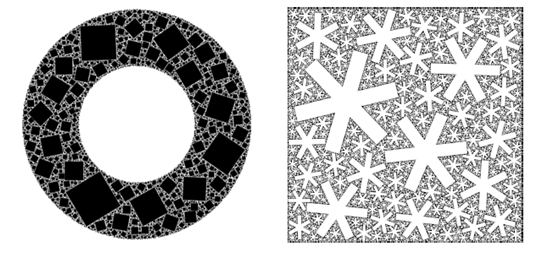
\includegraphics[scale = 1]{randomized1}
\end{figure}


Bubble$\&$Circle packing algorithms are widely used for mesh generation problems in finite element method. Shimada and Gossard \cite{27} proposed a method based on interbubble forces to provide close packaging of bubbles in desired geometrical shape. They define artificial interbubble forces to avoid collisions between bubbles and shape forces to keep the bubbles at the interior region of the desired shape. This idea is similar to the potential field based approaches in formation control problem since they both define artificial force components on individuals to cover a desired shape homogenously. The related interbubble forces are described at Figure \ref{interbubble_ref}. These forces have a nonlinear function of distance between the center of each bubbles and if this distance is larger than $l_o$, the interbubble forces are negative which means they attract each bubble towards the other ones. Interbubble forces increase while the distance between bubbles are decreasing to provide collision avoidance between bubbles. $l_o$ is the stable distance in which there is no interbubble force acting on bubble and it reaches an equilibrium point in the workspace.

\begin{figure}[H]
	\caption{Interbubble Forces \cite{27}} \label{interbubble_ref}
	\centering
	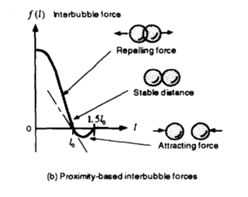
\includegraphics[scale = 0.3]{interbubble}
\end{figure}

The main idea is provide a close packing of bubbles which mimics a pattern of Voroni tessellation, corresponding to well shaped Delaunay triangles or tetrahedras.Figure \ref{tetrahedra} shows the corresponding voronoi polygons and delaunay triangles of a set of packed bubbles. The center of the cells in voronoi polygons are selected as the centers of the bubbles. Delaunay triangles corresponding to the set of uniformly packed of bubbles are well-shaped triangles \cite{27}. 

\begin{figure}[H]
	\caption{Uniform and Non-Uniform Node Spacing \cite{27}} \label{tetrahedra}
	\centering
	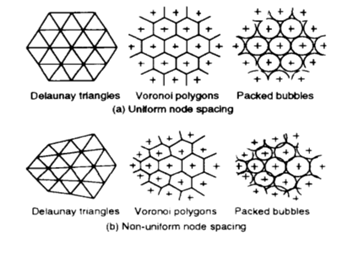
\includegraphics[scale = 0.35]{nodespacing}
\end{figure}

With the help of these interbubble forces, they provide an adaptive bubble packing algorithm for mesh generation. A result with a 2D shape is given at Figure \ref{mesh_genearation_ref}. At the end of 50 iterations, bubbles cover the desired shape with uniform spacing with the help of interbubble forces and the resultant delaunay triangulation corresponding to the set of packed bubbles are well-shaped triangles. 


\begin{figure}[H]
	\caption{Mesh Generation with Interbubble Forces \cite{27}} \label{mesh_genearation_ref}
	\centering
	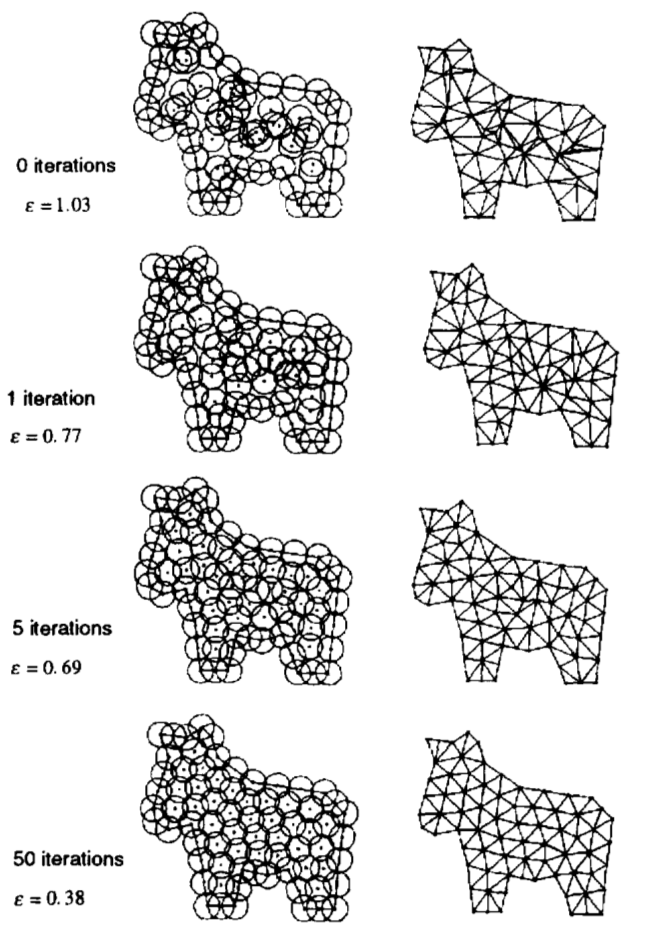
\includegraphics[scale = 0.4]{interbubble2}
\end{figure}

This approach can easily be augmented for different types and number of shapes to partition a complex geometrical shape with regular sets. It is possible to generate a mesh with different shapes which represents different types of agents in the swarm, rather than using bubbles with same radius. With this adaptation on the proposed method, it is possible to partition the desired shape into goal states which are subsets of different types of agents in the swarm with the help of interbubble forces. 

\section{Local Positioning Systems} \label{LPS_systems_ref}

Positioning systems are used to provide the required position data to the systems where it is desired to control the location of the mobile agent in the workspace. 
These systems fall into two main branches, global positioning systems and local positioning systems. Global positioning systems(GPS) has become increasingly popular for a couple of last decades for tracking location. In outdoor formation control applications this solution is used for positioning \cite{29}. It is a precise system depends on satellite based positioning mainly developed for direction finding and navigation.  Some of the problems encountered with the usage of GPS systems: (1) the signal from the satellites cannot penetrate to the indoor space so it doesn't perform in such areas, (2) it looses its precision in rich scattering environments such as urban areas \cite{19}.  A local positioning system can provide a position information where GPS systems are unavailable,with the usage of signaling beacons which are placed at the exactly known locations. In indoor formation control applications this kind of approach is used for positioning \cite{96}. 




\begin{figure}[H]
	\caption{Accuracy Statistics of Different Positioning Sources \cite{20}} \label{overview_position}
	\centering
	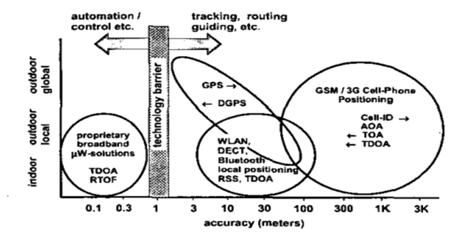
\includegraphics[scale = 0.4]{gps}
\end{figure} 

Figure \ref{overview_position} represents an overview of current positioning systems \cite{20}. Global positioning systems are widely used and they provide accuracies in the range of 3-30 meters. They further can operate in outdoor environments requiring radio signals from satellites. Differential GPS systems decrease these accuracy range below 3 meters with the help of additional local static beacons. GSM based solutions have the worst accuracy performance because they localize the nodes in the network by checking the relative signal strengths from different beacons, but they can perform in indoor environments partially \cite{20}.  Local positioning systems have the capability of working indoor environments because they use the signaling beacons which are placed at the exactly known locations \cite{20}. 

Local positioning systems has different system topologies illustrated in the Table \ref{different_top}.

\begin {table}[H]
\begin{center}
\newcommand{\wrap}[1]{\parbox{.40\linewidth}{\vspace{1.5mm}#1\vspace{1mm}}}
\caption {Local Posititioning Systems with Different System Topologies \cite{20}} \label{different_top} 
\begin{tabular}{ |c|c| } 
\hline
\wrap{Concept} &\wrap{Concept	Definition} \\
\hline
\wrap{Remote Positioning} &\wrap{Measurement from remote site to mobile device}\\
\hline
\wrap{Self Positioning}&\wrap{Measurement from mobile unit to usually fixed transponders(landmarks)} \\
\hline
\wrap{Indirect remote positioning}&\wrap{Self positioning system with data transfer of measuring result to remote site } \\
\hline
\wrap{Indirect self positioning}&\wrap{Remote positioning system with data transfer of measuring result to mobile unit} \\			
 \hline
\end{tabular}
\end{center}
\end{table}

Two main topologies are self positioning and remote positioning systems \cite{20}.  In a self positioning system, a mobile device finds its own position with the help of a predetermined reference such as a starting point or a beacon node with exactly known positions. On the other hand, in remote positioning systems a mobile node locates other objects' positions relative to its own position \cite{19}.   These two type of topologies can be converted to each other with the help of communications structures integrated on the devices to share the result of position measurement and thus indirect remote positioning and indirect self positioning system topologies can be implemented. Self positioning systems can be implemented to provide position data to the individual agents in formation control problems. The approach is to distribute the position data to the individual agents from a beacon node with exactly known positions. The individual agents which do not have a positioning sensor on their boards, measure their distance to these beacons and correct their position data with these external measurements. Beacons are assumed to have a GPS sensor on their boards for outdoor applications. They are assumed to have a special tag to locate them in an indoor environment with the help of external devices such as an E/O camera.




\subsection{Measurement Principles} \label{sssec:num1}
Local positioning systems can be used to provide position data in formation control problem by using robot networks. These systems differ mainly based on their measurement approaches which are the angle of arrival (AOA), received signal strength(RSS) and propagation-time based systems used in local positioning systems. 

\begin{figure}[H]
	\caption{Different Measurement Principles \cite{20}}
	\centering
	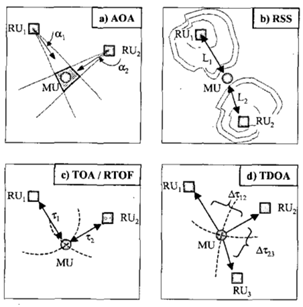
\includegraphics[scale = 0.4]{measurement}
\end{figure} 

Angle-of-arrival (AOA) systems use directional antennas to measure the bearing angle to the points located at known positions are measured. The position value of device can be calculated with the intersection of several measurements, but the accuracy is limited by shadowing and multipath reflections of radio signals \cite{20}. 

Received signal strength (RSS) systems calculate the distance value by taking the difference of the received signal power from the transmitted power. Some advanced propagation models are required to calculate the distance from the transmission loss in the air to eliminate the multipath fading and shadowing effects \cite{21}. 

Time based systems calculates the distance between measuring unit and signal transmitter with the help of propagation time like used in the global positioning systems generally. This process requires a perfect time synchronization between the mobile and stationary units \cite{20}.

In this thesis work, we implement a self positioning system in which every agent localize itself with the help of position beacons in the swarm with exactly known positions. The distance from the agents to these beacons in the swarm are assumed to be calculated with the help of a time of arrival(TOA) solution in which a node can calculate its distance to the transmitter beacon by measuring the difference between the timestamps of transmission and reception of the signal. 


\subsection{Trilateration Process} \label{Trilateration_Process_ref}

Trilateration process is used to determine the position of unknown locations with the help of distance measurement to known positions \cite{22}. In self positioning systems, the main approach is to calculate the position of mobile agents with the help of distance measurements to the beacons with exactly known positions. This position calculations are handled with trilateration process. It is widely used in wireless sensor network topologies and local positioning systems.  In theory, it is needed to have at least four beacon nodes to calculate an unknown position in 3D, and at least three beacon nodes to calculate an unknown position in 2D environment. But these worst case numbers are generally not sufficient to estimate an unknown position with a good accuracy due to errors on range calculations and synchronization problems. Figure \ref{trilateration_ref} demonstrates a simple trilateration process in 2D environment with the help of  three position beacons. Suppose a mobile device which tries to estimate its position with the help of local positioning system is at the red point in the figure. If it can measure its distance to the beacons named A,B and C with exactly known positions, it will be possible to estimate the unknown position of this mobile device with the same approach used in global positioning systems. 


\begin{figure}[H]
	\caption{Trilateration Process \cite{101}} \label{trilateration_ref}
	\centering
	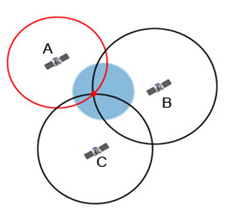
\includegraphics[scale = 1]{trilateration}
\end{figure}

